%*****************************************************************************************************            
%                               INSTITUT MINES-TELECOM, IMT ATlantique
%                         Département Mathematical & Electrical Engineering           
%                                     Technopôle de Brest-Iroise                   
%                                  CS 83818 - 29238 BREST Cedex 3                       
%            
%                                    **  Tous droits réservés **
%                                      
%
% NOM DU PROJET : TP LaTeX 006 / Modèle de rapport de recherche (validé par la DRI), de support de cours
% et de TP au format LaTeX avec les éléments de la charte graphique de la communication d'IMT Atlantique
%
% LIVRABLE : [ ] Memo, [ ] Résumé, [ ] Article, [ ] Code, [X] Rapport , [ ] Thèse, [ ] Cours/TP
%
% AUTEUR(s) : Thierry LE GALL (Dépt. MEE), Guillaume ANSEL (SC), Thomas GUILMENT (Dépt. SC)
%
% HISTORIQUE :
%
% Date          Nom(s)          Version  Description
% ------------  --------------- -------  ----------------------------------------------------------
% 12-mar-2015   T. LE GALL (SC) 0.0      création du document 
% 26-mar-2016   T. LE GALL (SC) 0.1      mise à jour : essai du package UTF8
% 26-sep-2016   G. ANSEL        0.2      mise à jour : ajout exemple utilisation TBannexe
%                                        ajout correction titres en majuscule dans sommaire
%                                        (cf BUGFIX_TITRES_SOMMAIRE dans imta.sty)
%                                        changement polices utilisées
% 09-jan 2017   T. LE GALL (SC) 0.3      mise à jour : évolution du modèle de TB vers IMT Atlantique
% 03-fev 2017   G. ANSEL        0.4      mise à jour : modifications pour adaptation à version 1.5 du package imta
%                                        ajout méta-données PDF
% 14-fev-2017   T. GUILMENT     0.5      mise à jour : ajout package fancyhdr pour entêtes et pieds de page
%                                        changement style titres
% 16-fev-2017   G. ANSEL        0.6      mise à jour : modifications pour version 1.6 package imta
%                                        ajout style de page IMTAfancy pour entêtes et pieds de page
%                                        remplacement \listoffigures et \listoftables par \IMTAlistefigures
%                                        et \IMTAlistetableaux
% 17-fev-2017   G. ANSEL        0.7      mise à jour : déplacement définition style IMTAfancy dans imta.sty
%                                        définition commande \IMTAfooter pour personnaliser le pied de page
%                                        en bas à gauche
% 21-fev-2017   T. LE GALL (SC) 0.8      mise à jour : ajout d'un exemple de n° de contrat de recherche
%                                        (pied de page) et vérification de la compilation du document 
% 28-fev-2017   G. ANSEL        0.9      mise à jour : ajout exemple d'utilisation de l'option copyright
%                                        du package imta (informations copyright sur quatrième de couverture)
% 06-fev-2017   T. LE GALL (SC) 1.0      mise à jour : ajout de définitions d'ensembles mathématiques et exemple
%                                        d'édition de bloc dans le texte.  Ajout de la mention FIN DE FICHIER. 
%                                        Test de compilation avec imta.sty (v2.3) = PASS (0 errors, 0 warnings).
% 06-avr-2017   T. LE GALL (SC) 1.1      mise à jour : ajout du type de document et du numéro de rapport
%                                        de recherche en tant que paramètre du document et affichage des
%                                        informations en première de couverture (suite à demande de la DRI)
% 03-aoû-2017   T. LE GALL (SC) 1.2      mise à jour : exemple de section de texte sur deux colonnes et équations
%                                        dans deux blocs adjacents de style Beamer
% 09-aoû-2017   T. LE GALL (SC) 1.3      mise à jour : ajout des équations (matrices, vecteurs)
% 11-sep-2017   T. LE GALL (SC) 1.4      mise à jour : attribution du n°ISSN 2556-5060 pour les rapports de recherche
% 22-sep-2017   G. ANSEL        1.5      mise à jour : ajout d'un exemple d'insertion de tableau
% 25-sep-2017   T. LE GALL      1.6      mise à jour : légende du tableau et n° de version du modèle en page de garde
%                                        + tests de non-négression du modèle (env. Win 7) suite à BUGFIX_21092017_1
%                                         et BUGFIX_21092017_2 dans le fichier imta.sty v2.8 et v2.9
% 27-nov-2018   G. ANSEL        1.7      mise à jour : modifications pour passage en version 3.5 du package imta
% 21-jan-2019   T. LE GALL (SC) 1.8      mise à jour : couverture : type de document au-dessus de titre et liste
%                                        des auteurs et contributeurs sous le titre + tests de compilation (Win10)
%                                        + tests de compilation (UBUNTU 18.04 LTS)
% 10-mai-2020  T. LE GALL (SC)  1.9      mise à jour : ajout d'exemples supplémentaires (équations) 
% 25-jan-2021  T. LE GALL (MEE) 2.0      mise à jour : département Mathematical & Electrical Engineering                                      
%
%
% NOTES/COMMENTAIRES :
%
% - Exemple de rapport scientifique au format IMT Atlantique sous LaTex avec insertion de formules,
%   figures, ref. biblio, hyperliens, signets, renvois actifs, surlignage des formules. Le fichier
%   d'édition tp_latex_006.tex utilise le fichier de style imta.sty. Cf. fichier lab_006_readme.txt
%   situé sous le répertoire lab_006.
%
% REFERENCES :
%
% - cf. bibliographie
% 
%***********************************************************************************************

%-----------------------------------------------------------------------------------------------
%                                    DEBUT DU FICHIER D'EDITION
%-----------------------------------------------------------------------------------------------

\documentclass[11pt,a4paper]{article}

\usepackage{babel}
\usepackage[utf8]{inputenc}
\usepackage[T1]{fontenc}
\usepackage{float}
\usepackage{newtxtext} % Police pour texte
\usepackage{newtxmath} % Police pour formules
\usepackage{textcomp}
\usepackage{graphicx}
\usepackage{amsmath}
\usepackage{microtype}
\usepackage{subcaption}
\usepackage{multirow}
\usepackage{pythontex} 
\usepackage{listings}
\usepackage{biblatex}
 \bibliography{bibliography.bib}

\usepackage{framed}	% Permet de surligner les résultats importants
\newcommand{\citationneeded}[1][]{\textsuperscript{\color{blue} [citation needed]}}

% Charte graphique de IMT Atlantique
% L'option "version" affiche la menion "Document version x" sur la première de couverture
% Le numéro de version est paramétrable via la commande "\version"
% L'option "copyright" affiche la mention "© IMT Atlantique ..." sur la quatrième de couverture
% Les informations de copyright sont paramétrables via les commandes \IMTAanneecopyright, \IMTAdepotlegal, \IMTAissn

\usepackage[copyright]{../sty/imta} % édition avec copyright (et n°ISSN) en 4eme de couverture
%\usepackage{../sty/imta}	% édition sans copyright (et n°ISSN) en 4eme de couverture

% Signets et hyperliens (à charger en dernier)
\usepackage[colorlinks=true,linkcolor=black,urlcolor=blue,citecolor=IMTAbleu]{hyperref} 

%----------------- Métadonnées du PDF (facilite le travail des moteurs de recherche) -----------
\hypersetup{
	pdfinfo = {
		Author = {<Martina María BALBI ANTUNES>; <Mateo BENTURA LARREGUI>; <Ezequiel Tomás CENTOFANTI>; <Kevin MICHALEWICZ>},
		Title = {<Machine Learning Project - Report>},
		Keywords = {<Machine Learning>; ...}
	}
}

%--------------------------- Définition du contenu du pied de page ----------------------------

% Le pied de page contient par défaut le titre du document.
% Il peut être remplacé en décommentant l'une des lignes ci-dessous

%\IMTAfooter{Modèle de document \LaTeX{} IMT Atlantique} % Exemple de remplacement par un autre texte
\IMTAfooter{\thereportnumber} % Utilisation du numéro de rapport de recherche

%-------------------- Informations de copyright pour quatrième de couverture ------------------
%          (uniquement si l'option "copyright" est présente pour le package imta)

% Les lignes ci-dessous permettent de remplacer manuellement le mois et l'année
% d'édition pour le dépot légal si nécessaire. Par défaut, le mois et l'année
% courants lors de la compilation du document sont utilisés

\IMTAanneecopyright{2021}
\IMTAdepotlegal{Septembre 2017}

%-------------------------------------- Do not modify -----------------------------------------
																									
% le numéro ISSN est communiqué par la BNF à la DRI. N°fixé par la BNF en
% fonction du type de document. Ne concerne que la collection des rapports
% de recherche (et pas les autres types de document utilisant ce modèle).
\IMTAissn{2556-5060}

%----------------------------------- End of do not modify -------------------------------------

%----------------- Définitions d'ensembles et d'opérateurs mathématiques ----------------------

\def\Cset{\mathbb{C}} % complexes
\def\Hset{\mathbb{H}} % hilbert
\def\Nset{\mathbb{N}} % entiers naturels
\def\Qset{\mathbb{Q}} % rationnels
\def\Rset{\mathbb{R}} % reels
\def\Zset{\mathbb{Z}} % entiers relatifs
\def\Dset{\mathbb{D}} % disque unite ouvert
\def\Eset{\mathbb{E}} % esperance mathematique

%-------------------------------------- FIN DES DEFINITIONS ----------------------------------

\begin{document}

%---------------------------------------------------------------------------------------------
%                                   PAGE DE TITRE (please modify)
%---------------------------------------------------------------------------------------------

% Type de document
%\DocumentType{<Type de document>}  
\DocumentType{TAF MCE - UE A}
%\DocumentType{Document support de BE et de TP}
%\DocumentType{Support de cours}
%\DocumentType{Support de TP}
%\DocumentType{Mémoire technique}


% Numéro de rapport de recherche (à remplacer)
% Commenter la ligne ci-dessous si le document n'est pas un rapport de recherche
%\ReportNumber{}


\entity{\textbf{\large{IMT Atlantique}}\\
% Dépt. Automatique productique et informatique\\
% Dépt. Électronique\\ 
 Départament Informatique\\ 
%Dépt. Image \& traitement de l'information\\
%Dépt. Langues \& culture internationale\\ 
%Dépt. Logique des usages, sciences sociales \& sciences de l'information\\ 
%Dépt. Micro-ondes\\ 
%Dépt. Optique\\
%Dépt. Physiques subatomiques et technologies\\
%Dépt. Sciences sociales et de gestion\\
%Dépt. Mathematical \& Electrical Engineering\\
%Dépt. Systèmes énergétiques et environnement\\
%Dépt. Systèmes réseaux, cybersécurité et droit du numérique\\
Technopôle de Brest-Iroise - CS 83818\\
29238 Brest Cedex 3\\
%Téléphone: +33 (0)2 29 00 13 04\\
%Télécopie: +33 (0)2 29 00 10 12\\
%4, rue Alfred Kastler\\
%CS 20722\\
%44307 Nantes Cedex 3\\
%Téléphone: +33 (0)2 51 85 81 00\\
%Télécopie: +33 (0)2 99 12 70 08\\		
%2, rue de la Châtaigneraie\\
%CS 17607\\
%35576 Cesson Sévigné Cedex\\
%Téléphone: +33 (0)2 99 12 70 00\\
%Télécopie: +33 (0)2 51 85 81 99\\
%10, avenue Édouard Belin\\
%BP 44004\\
%31028 Toulouse Cedex 04\\
%Téléphone: +33 (0)5 61 33 83 65\\		
URL: \textbf{\href{http://www.imt-atlantique.fr/}{www.imt-atlantique.fr}}
}

%\docdescription{<Destinataire : >}

\title{Machine Learning Project - Report}
%\title{Étude d'une forme d'onde pour communications longues-distances par le canal acoustique sous-marin}

\author{
	Martina María BALBI ANTUNES\and
	Mateo BENTURA LARREGUI\and
	Ezequiel Tomás CENTOFANTI\and
	Kevin MICHALEWICZ
}


% Numéro de version du document, affiché sur la couverture
% Commenter cette ligne pour ne pas faire apparaître la version du document.
%\version{2.0}


%------------------------------------------ Do not modify ------------------------------------
\IMTAfrontcover
\pagestyle{IMTAfancy} % Changement du style de page pour avoir en-tête et pied de page
%--------------------------------------- End of do not modify --------------------------------

%% Affichage des listes et tables.
\IMTAsommaire
\newpage
\IMTAlistefigures  % commenter pour ne pas avoir la liste des figures
\IMTAlistetableaux   % commenter pour ne pas avoir la liste des tables
\newpage
%---------------------------------------------------------------------------------------------
%                                   INTRODUCTION (please modify)
%---------------------------------------------------------------------------------------------

\section{Introduction} 

This report describes our final work for the UE Machine Learning of IMT Atlantique. Throughout it, we present several techniques to solve the classification problem for the Banknote Authentication and Chronic Kidney Disease datasets.

Some of the objectives of this project are to use standard development tools, work collaboratively, develop good programming practices and become familiar with Machine Learning datasets.

First of all, the datasets will be cleaned and normalized. We will proceed by using the Principal Component Analysis (PCA) technique for dimensionality reduction. After that, the following Machine Learning methods will be applied: K-nearest Neighbors (KNN), Support Vector Machines (SVM), Gaussian Mixture Models (GMM) and Neural Networks (NN). Finally, the results will be analyzed, a section on good programming practices will be included and conclusions will be drawn. The complete code and the Git log can be found in the appendix.

\section{Datasets}

\subsection{Banknote Authentication}

The Banknote Authentication dataset \cite{ba} contains 1372 records of several banknotes. The data present was extracted from images of each banknote being some genuine and some fake. These images are of $400x400$ pixels, gray-scaled and with a resolution of about $660 dpi$. Then, the images were transformed using the Wavelet Transform tool and the following information, the features present in the dataset, were extracted from them: Variance, Skewness, Curtosis and Entropy.

\subsubsection{Preprocessing}
Fortunately, this dataset is $100\%$ complete, meaning that all examples contain all the features and they are all already floats. Therefore, the dataset was only imported, the column names were added for simplicity, the labels were extracted and finally the data was normalized. 

\subsection{Chronic Kidney Disease}

The Chronic Kidney Disease dataset \cite{ckd} was obtained after medical studies in India which lasted two months. 25 features, being some of them categorical and other numerical, may help to predict if a given patient possesses the disease or not. There are 400 rows.

\subsubsection{Preprocessing}

The data preprocessing stage for this dataset was more complicated than in the previous case. The first thing to do was to convert the data in the \textit{packed\_cell\_volume}, \textit{white\_blood\_cell\_count} and \textit{red\_blood\_cell\_count} columns to numeric type, leaving \textit{NaNs} in case of conversion errors. Afterwards, categorical and numerical columns were clearly separated. In this sense, \textit{NaN} values were replaced by the mean of valid amounts from the same feature in the case of numerical columns, and by the the most frequent binary label for categorical columns. In addition, tabs and blanks had to be removed.

At this point, the normalization of the numerical features was performed and the categoricals were casted to \textit{True} or \textit{False} with pandas \textit{get\_dummies()} method. Finally, the classes $y$ (diseased or not) were extracted and return as a separate vector.

\section{Principal Component Analysis}

Principal Component Analysis (PCA) is an unsupervised learning method that simplifies the complexity of high-dimensional sample spaces while preserving their information.

Using \textit{plot\_pca\_correlation\_graph} it was possible to obtain the correlation circles of the different datasets, which are shown in Figure~\ref{pca_circles}.

\begin{figure}[h]
\centering
\begin{subfigure}{.5\textwidth}
  \centering
  \includegraphics[width=0.9\linewidth]{img/pca_circles_ba.png}
  \caption{Banknote Authentication dataset.}
  \label{fig:sub1}
\end{subfigure}%
\begin{subfigure}{.5\textwidth}
  \centering
  \includegraphics[width=0.9\linewidth]{img/pca_circles_kd.png}
  \caption{Kidney Disease dataset.}
  \label{fig:sub2}
\end{subfigure}
\caption{Correlation circles for both datasets.}
\label{pca_circles}
\end{figure}

The easiest case to interpret due to the number of features is the Banknote Authentication dataset. It is evident that skewness and curtosis can be described by the first dimension of PCA. The same can be said for variance and entropy looking at the second component. Furthermore, by analyzing the direction of the arrows it is possible to understand the correlations of the features. Finally, the percentage of the information (variance) represented by each of the two components can be read on the axes.

PCA was done in a very similar way in both datasets, except that in Kidney Disease categorical variables were not processed because many authors recommend excluding them in this regard.

After gaining an intuition regarding how the features and their correlations behave, different component values for the PCA algorithm were tested. It was chosen to retain more than 85\% of the variance in both cases. In particular:
\begin{itemize}
  \item For the Banknote Authentication dataset 2 components that represent 0.87 of the original variance were considered.
  \item For the Kidney Disease dataset 10 numerical components that represent 0.92 of the original variance were considered.
\end{itemize}

New datasets with dimension reduction were obtained at the output, being ready to be treated with the Machine Learning algorithms that will be described below.

\section{K-Nearest Neighbors}

The K-Nearest Neighbors classifier is an algorithm based on a set of data for training and for evaluation of a model, of a supervised type. The latter means that the training data includes the desired solution (labels).

This classifier is a method that considers the samples closest to the one to be predicted. Then, from these samples, it classifies the new data of interest based on the majority of data around it. This closeness depends on the variable K (integer), which refers to the number of neighbors to be considered.

In order to choose the best value of $K$, the accuracy of the model was tested for $K=1$ to $K=7$. The value of $K$ that yielded the best results was used for the final model. These results are presented in the following Table \ref{tab:knn_chose_k}:

\begin{table}[h!]
    \centering
    \begin{tabular}{|c|c|c|c|c|c|c|c|}
    \hline
    \bf & \bf K=1  & \bf K=2  & \bf K=3  & \bf K=4  & \bf K=5 & \bf K=6 & \bf K=7 \\\hline
    \bf banknote-authentication  & 100.00 & 100.00 & 100.00  & 100.00   & \bf 100.00 & 99.51 & 99.51 \\\hline
    \bf kidney-disease & 95.00 & 95.00 & 95.00 & 95.00 & \bf 96.67 & 95.00 & 95.00\\\hline
    \end{tabular}
    \caption{Accuracy in both datasets of KNN for different values of K.}
    \label{tab:knn_chose_k}
\end{table}

Taking into consideration the results presented above, the best value of $K$ appears to be $K=5$. The confusion matrix for each dataset is shown in Figure~\ref{cm_knn}.

\begin{figure}[H]
\centering
\begin{subfigure}{.5\textwidth}
  \centering
  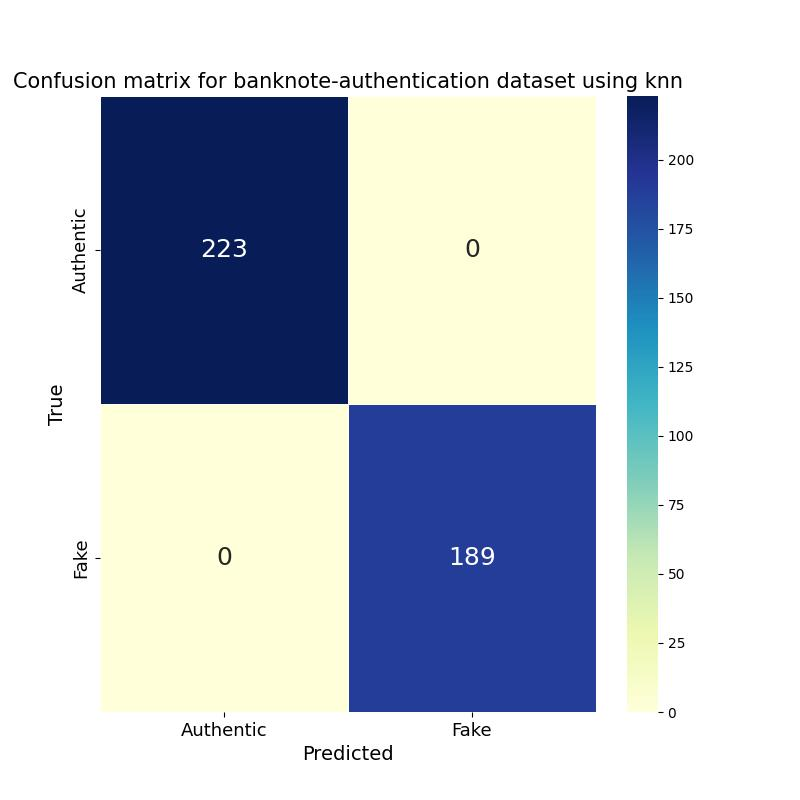
\includegraphics[width=0.9\linewidth]{img/Confusion_Matrix_banknote-authentication_knn.jpg}
  \caption{Banknote Authentication dataset.}
  \label{fig:sub1}
\end{subfigure}%
\begin{subfigure}{.5\textwidth}
  \centering
  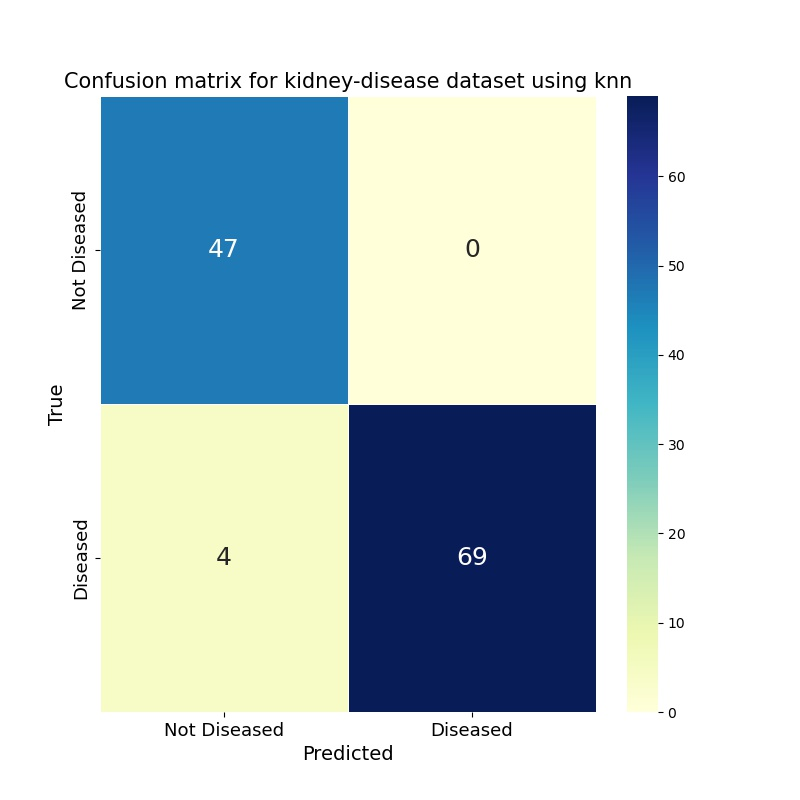
\includegraphics[width=0.84\linewidth]{img/Confusion_Matrix_kidney-disease_knn.jpg}
  \caption{Kidney Disease dataset.}
  \label{fig:sub2}
\end{subfigure}
\caption{Confusion matrices for classification of both datasets using KNN ($K=5$).}
\label{cm_knn}
\end{figure}

This model correctly classifies all examples of the banknote authentication dataset and almost all of the kidney disease dataset. However, these 4 misclassified examples of the kidney disease are not unimportant, since they represent 4 patients that were diagnosed as not diseased when they actually had a kidney disease. For this type of applications, these kind of errors are very problematic. Therefore, it is to be concluded that while this model appears to be excellent for proving the authenticity of banknotes, it is not very good for diagnosing patients with kidney disease. 

\section{Support Vector Machines}

Support Vector Machines is a supervised learning technique that searches for a hyperplane to separate two classes of points, including a margin to maximize the minimal distance. It is a quite simple calculation as it depends just on the support points. Given the case in which the clouds are not linearly separable, we can limit the error by adding the $\xi_i$ coefficients that represent the distance between wrongly classified individuals and the margin we are willing to accept. Another option is to introduce the \textit{Kernel Trick} and work with transformations to spaces of larger dimensions. 

The scikit-learn library was used and the model was fitted by using \texttt{sklearn.svm.SVC()} with default parameters.

The confusion matrix for each dataset is shown in Figure~\ref{cm_svm}.

\begin{figure}[H]
\centering
\begin{subfigure}{.5\textwidth}
  \centering
  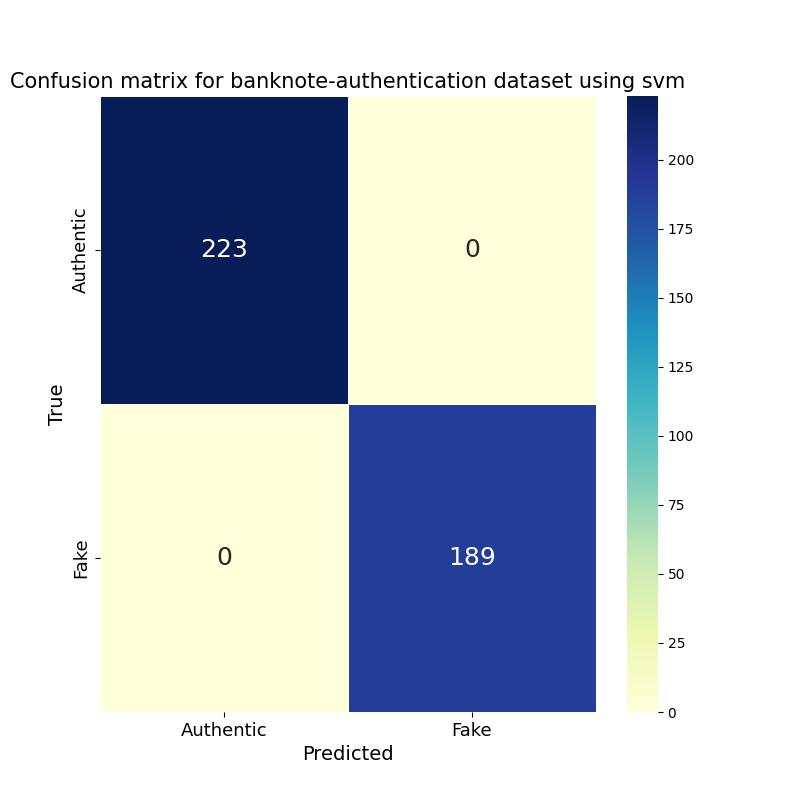
\includegraphics[width=0.9\linewidth]{img/Confusion_Matrix_banknote-authentication_svm.jpg}
  \caption{Banknote Authentication dataset.}
  \label{fig:sub1}
\end{subfigure}%
\begin{subfigure}{.5\textwidth}
  \centering
  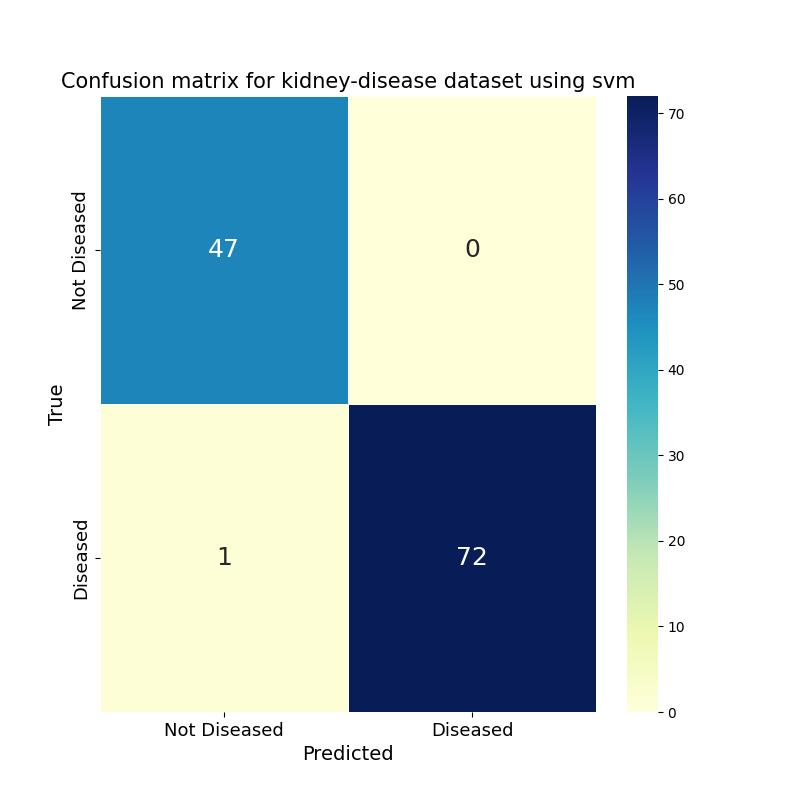
\includegraphics[width=0.9\linewidth]{img/Confusion_Matrix_kidney-disease_svm.jpg}
  \caption{Kidney Disease dataset.}
  \label{fig:sub2}
\end{subfigure}
\caption{Confusion matrices for classification of both datasets using SVM.}
\label{cm_svm}
\end{figure}

The results are fairly acceptable due to the fact that there are hits for both datasets in all predictions, except in one case corresponding to a false negative in Kidney Disease.

\section{Gaussian Mixture Models}
We applied the technique known as Gaussian Mixture Models (GMM) to both datasets. This is an unsupervised model that fits data to a mixture of Gaussian distributions using the expectation-maximization algorithm, but a supervised approach was taken: two Gaussian mixture model are trained, one for each class in order to model their probability distribution. In order to make a prediction, the test samples' likelihood are evaluated using both models and the one with a greater likelihood is chosen.

The resulting parameter of this classifier is the number of mixture components used to model the data in each class. In the case of the BA dataset, the number used was 2 mixture components, where as only one sufficed for the KD dataset (i.e. each class is modelled as a Gaussian distribution).

The model was implemented using the class \texttt{GaussianMixture} from the scikit-learn module \texttt{sklearn.mixture}.

The resulting confusion matrices for this model are shown in Figure~\ref{cm_gmm}. We conclude this is a fairly good result, given the simplicity of this classifier.

\begin{figure}[H]
\centering
\begin{subfigure}{.5\textwidth}
  \centering
  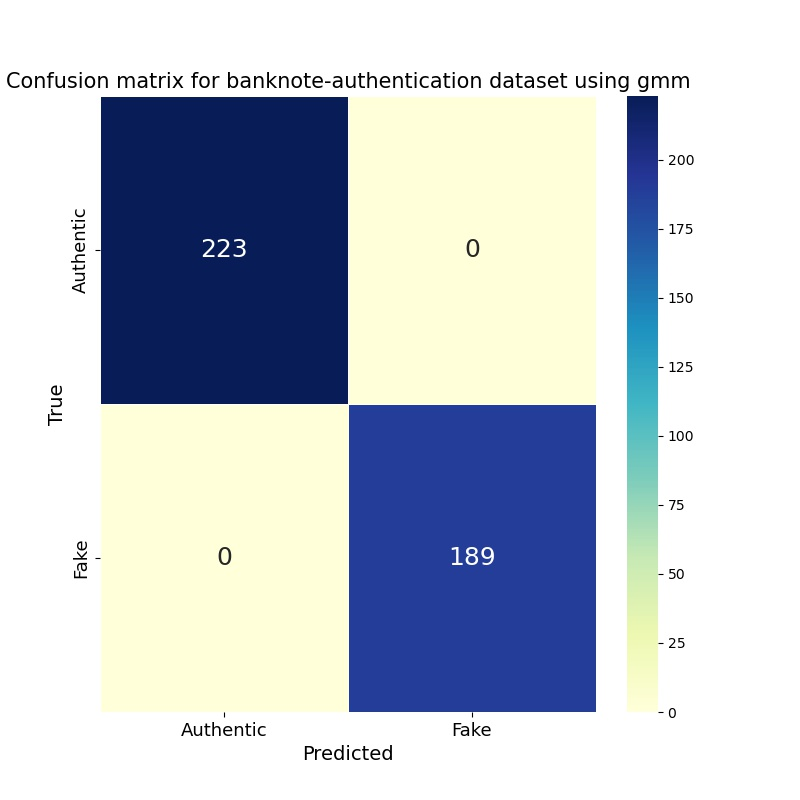
\includegraphics[width=0.9\linewidth]{img/Confusion_Matrix_banknote-authentication_gmm.jpg}
  \caption{Banknote Authentication dataset.}
  \label{fig:sub1}
\end{subfigure}%
\begin{subfigure}{.5\textwidth}
  \centering
  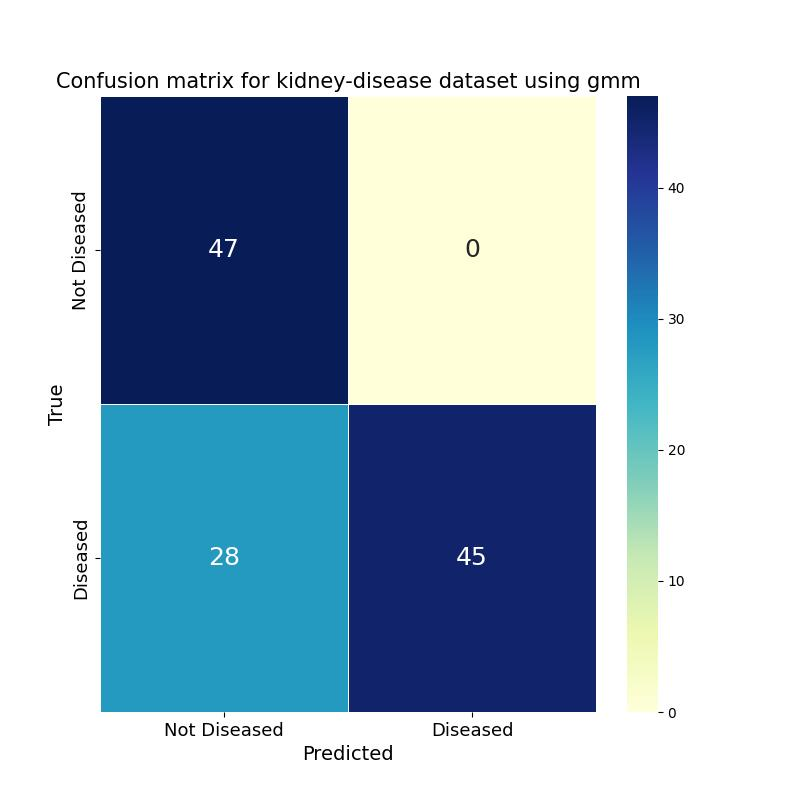
\includegraphics[width=0.9\linewidth]{img/Confusion_Matrix_kidney-disease_gmm.jpg}
  \caption{Kidney Disease dataset.}
  \label{fig:sub2}
\end{subfigure}
\caption{Confusion matrices for classification of both datasets using GMM.}
\label{cm_gmm}
\end{figure}

\section{Neural Networks}

Another method used for classification is the application of neural networks. For both datasets (CKD and BA) the data consists of a set of features without any apparent spatial relationship, therefore fully connected neural networks are used and not convolutional or other types. 

In general, such methods tend to tackle much more complex and higher dimensional problems. Yet we can easily implement them for this classification problem. 

The most basic hyperparameters to determine in this type of network are the number of layers to be used and the number of nodes or neurons per layer. This is by no means a simple task in general and in most cases the answer is a bit of experience and experimentation. 

Since the problem to be solved is relatively simple, it is tested with a single layer, whose number of inputs will be the number of features according to the dataset and with a single output. The number of parameters to train is equal to the number of features plus one, the latter corresponding to the bias of the output neuron. In this approach we are trying to separate the data by a hyperplane in feature space.

For both datasets the binary cross-entropy is used as loss function and the optimisation method used is stochastic gradient descent. The number of epochs was set at 80 for both datasets with a learning rate of 0.05. A validation set of size 25\% of the training set is used to determine the number of epochs. Figure~\ref{lossesNN} shows the losses over the training and validation sets for each epoch for each dataset. 

\begin{figure}[H]
\centering
\begin{subfigure}{.5\textwidth}
  \centering
  \includegraphics[width=1\linewidth]{img/Losses_banknote-auth.jpg}
  \caption{Banknote Authentication dataset.}
  \label{fig:sub1}
\end{subfigure}%
\begin{subfigure}{.5\textwidth}
  \centering
  \includegraphics[width=1\linewidth]{img/Losses_kidney-disease.jpg}
  \caption{Kidney Disease dataset.}
  \label{fig:sub2}
\end{subfigure}
\caption{Loss over training and validation sets for each epoch.}
\label{lossesNN}
\end{figure}

The number of epochs is chosen approximately where the loss function does not decrease considerably with increasing number of epochs. Normally we would observe that at some point the validation loss increases while the training loss continues to decrease slightly, at this point we would start to overfit the data and we should stop, but we will not see that in this case, as the model is too simple for overfitting. 

\begin{table}[h!]
    \centering
    \begin{tabular}{|c|c|}
    \hline
    \bf & \bf Accuracy \\\hline
    \bf banknote-authentication  & 98.00  \\\hline
    \bf kidney-disease & 99.00 \\\hline
    \end{tabular}
    \caption{Accuracy in both datasets for NN classification.}
    \label{tab:NN_accuracy}
\end{table}

The results of this method are presented in Table \ref{tab:NN_accuracy} and the confusion matrix is shown in Figure~\ref{cm_nn}. The two neural networks correctly classify data from both datasets, even with the simplest possible network model.

\begin{figure}[H]
\centering
\begin{subfigure}{.5\textwidth}
  \centering
  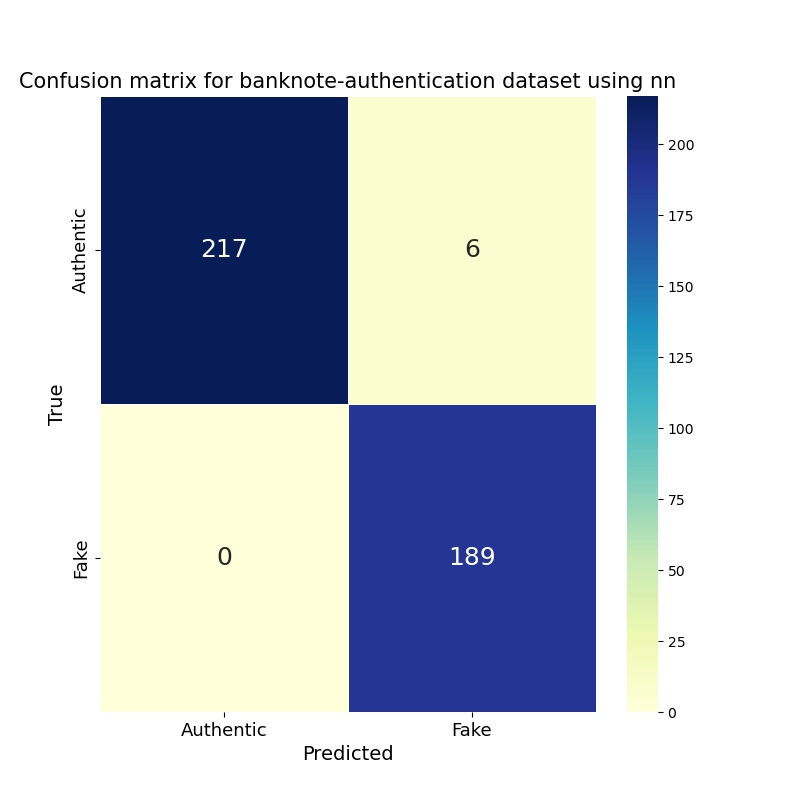
\includegraphics[width=1\linewidth]{img/Confusion_Matrix_banknote-authentication_nn.jpg}
  \caption{Banknote Authentication dataset.}
  \label{fig:sub1}
\end{subfigure}%
\begin{subfigure}{.5\textwidth}
  \centering
  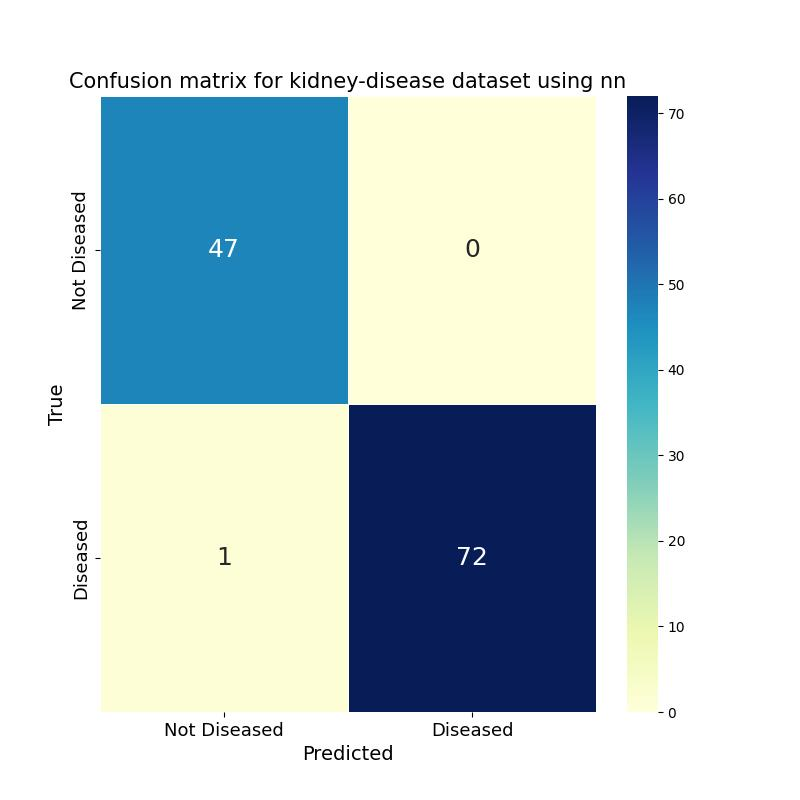
\includegraphics[width=1\linewidth]{img/Confusion_Matrix_kidney-disease_nn.jpg}
  \caption{Kidney Disease dataset.}
  \label{fig:sub2}
\end{subfigure}
\caption{Confusion matrices for classification of both datasets using NN.}
\label{cm_nn}
\end{figure}


\section{Results}
In order to evaluate the performance of the four models used to classify, the confusion matrices were generated (as seen in each section). Also, precision, recall and the F1-scores were computed. These scores are presented in the following Table \ref{tab:scores}:

\begin{table}[h!]
\centering
\begin{tabular}{|c|cccc|cccc|}
\hline
\multirow{2}{*}{}  & \multicolumn{4}{c|}{\textbf{Banknote Authentication}}                                                                    & \multicolumn{4}{c|}{\textbf{Kidney Disease}}                                                                            \\ \cline{2-9} 
                   & \multicolumn{1}{c|}{\textbf{KNN}}  & \multicolumn{1}{c|}{\textbf{SVM}} & \multicolumn{1}{c|}{\textbf{GMM}} & \textbf{NN} & \multicolumn{1}{c|}{\textbf{KNN}} & \multicolumn{1}{c|}{\textbf{SVM}} & \multicolumn{1}{c|}{\textbf{GMM}} & \textbf{NN} \\ \hline
\textbf{Precision} & \multicolumn{1}{c|}{1.00}          & \multicolumn{1}{c|}{1.00}         & \multicolumn{1}{c|}{1.00}         & 0.97        & \multicolumn{1}{c|}{1.00}         & \multicolumn{1}{c|}{1.00}         & \multicolumn{1}{c|}{1.00}         & 1.00        \\ \hline
\textbf{Recall}    & \multicolumn{1}{c|}{1.00}          & \multicolumn{1}{c|}{1.00}         & \multicolumn{1}{c|}{1.00}         & 1.00        & \multicolumn{1}{c|}{0.95}         & \multicolumn{1}{c|}{0.99}         & \multicolumn{1}{c|}{0.93}         & 0.96        \\ \hline
\textbf{F1-score}  & \multicolumn{1}{c|}{1.00} & \multicolumn{1}{c|}{1.00}         & \multicolumn{1}{c|}{1.00}         & 0.98        & \multicolumn{1}{c|}{0.97}         & \multicolumn{1}{c|}{0.99}         & \multicolumn{1}{c|}{0.96}         & 0.98        \\ \hline
\end{tabular}
\caption{Scores used to evaluate the classifiers.}
\label{tab:scores}
\end{table}

As it can be seen in the table above, all models performed very well in both datasets.

\section{Good Programming Practices}

This work included a collaborative development of Machine Learning functions with an active use of Git. For the code to be readable, easily interpretable by members of the same group and third parties, and for the different modules to have a reasonable organization, it was necessary to adopt good programming practices. These will be detailed hereafter:

To make the code look as homogeneous as possible, we decided to use the PEP 8 Python Code Style Guide\footnote{https://www.python.org/dev/peps/pep-0008/} before starting to program. Among other things, there one can see how to place function arguments, the correct format for loops, naming conventions and imports.

On the other hand, in order to make each function instantly understandable, a long comment was included in each of them detailing: what is its role, which are the input arguments and what it returns.

As already mentioned, the project was divided into modules in terms of code. It includes a main program \textit{main.py} that uses \textit{clean\_normalize.py} to clean and normalise the input datasets, \textit{ml\_functions.py} contains the functions associated with the Machine Learning methods, \textit{tools.py} carries general tools such as the lines of code that have to do with plotting the confusion matrices. This organisation made it easy to work through Git in a collaborative way. In this sense, making recurring and explanatory commits was the adopted approach.

In addition, a \textit{.txt} file with the Python modules required to run the project was included as well as a \textit{README.md} to guide users on being able to get results on the command line using our code.


%---------------------------------------------------------------------------------------------
%                                   CONCLUSIONS (please modify)
%---------------------------------------------------------------------------------------------
\section{Conclusions}

In this work, two classification problems were solved by applying different machine learning techniques. First, a study of both problems was carried out in order to understand them and to be able to propose different solutions. Both problems consist of binary classification of data having corresponding real values, i.e. it is a supervised learning problem. The objective is to generate a function or inference rule that allows to assign a class to a new data point never seen before, and ideally that this class is the correct one.

The first step consists of handling the data, which may be encoded in a csv file or other type of file, it is necessary to clean and normalize the data, then we should analyse its structure in order to propose methods to solve the problem. The method applied is PCA, principal component analysis, it gives us the best projection on a lower dimensional subspace in terms of information maintenance, i.e. maximising the variance of the data. In this way we can reduce the number of relevant dimensions of the data by reducing the number of parameters of the solutions to be applied and by reducing the computational effort. 

Four methods are proposed to solve both problems: K-Nearest Neighbors, Support Vector Machines, Gaussian Mixture Models and Neural Networks. All the methods used gave relatively good results. It is important to understand the notion of the term "relatively good", because depending on the problem we can tolerate a given number of errors of one of the two types. For example in the case of kidney disease screening, false alarm errors could be tolerated but not miss errors (this is just an example without medical basis); nor would we want to declare a fake bank note as authentic. If we wanted to determine this rate with greater precision we would require a larger number of data points.

Another crucial axis of this project, and perhaps the most important in academic terms, is the adaptation to collaborative work and version control through the git tool. This project allowed us to practice our teamwork skills and to reinforce good programming practices in this type of collaborative work.

%--------------------------------------- DEBUT DES ANNEXES --------------------------------------
\newpage
\begin{IMTAannexes}
	
%-------------------------------------------- ANNEXE 1  -----------------------------------------
	
\IMTAannexe{Git Log}\label{sec:S_ANN_EX}

\begin{verbatim}
commit 5771c9ff3797ec1a5aafa79307505c91b08c736f
Author: Martina Balbi <martina.balbi14@gmail.com>
Date:   Wed Dec 15 12:25:20 2021 +0100

    implemented f1 scores

commit 220ee7f6de5a9688e9e8b85f91c6fc156d82d121
Merge: afd3be8 655db45
Author: Martina Balbi <martina.balbi14@gmail.com>
Date:   Wed Dec 15 11:51:18 2021 +0100

    Merge branch 'main' of https://github.com/kevinmicha/ML-IMTA-Project

commit afd3be81c47e37de9887b3c6c7d7cacbe2031998
Author: Martina Balbi <martina.balbi14@gmail.com>
Date:   Wed Dec 15 11:48:55 2021 +0100

    implemented f1 scores

commit 655db45e6f88195d3f372dfd26d2122261ec033b
Author: Martina Balbi <martina.balbi14@gmail.com>
Date:   Wed Dec 15 11:48:55 2021 +0100

    Merge branch 'main' of https://github.com/kevinmicha/ML-IMTA-Project

commit ebb3d16cc89f35b3b6bb8bce791b21b8a0e1844e
Author: Mateo Bentura <mateo.bentura-larregui@imt-atlantique.net>
Date:   Tue Dec 14 18:12:46 2021 +0100

    supervised GMM implementation

commit 478ba8678d787544932198efe6d407adb6852146
Author: Mateo Bentura <mateo.bentura-larregui@imt-atlantique.net>
Date:   Mon Dec 13 17:54:00 2021 +0100

    fixed function comment

commit 361a74c99107fc438c7eb9266747dd06abf0efea
Author: Mateo Bentura <mateo.bentura-larregui@imt-atlantique.net>
Date:   Mon Dec 13 17:47:26 2021 +0100

    plotted GMM covariances using PCA to gain insight into bad results

commit 1f3a9030359b3e03d0153c333829afacd435b4a9
Author: kevinmicha <kmichalewicz@fi.uba.ar>
Date:   Fri Dec 10 12:12:30 2021 +0100

    new plots

commit 22a44717b046a01b31b9c05041fd982b24e3f629
Author: kevinmicha <kmichalewicz@fi.uba.ar>
Date:   Fri Dec 10 12:12:20 2021 +0100

    confusion matrix pipeline is ready

commit fc231078ab63f3a2e20a97726e013e1467edc82e
Author: kevinmicha <kmichalewicz@fi.uba.ar>
Date:   Fri Dec 10 11:56:15 2021 +0100

    adding loss plots for nn

commit a0647b6229eaab6c2c0ec83fa4fa44fd20fb9bbe
Author: kevinmicha <kmichalewicz@fi.uba.ar>
Date:   Fri Dec 10 11:55:57 2021 +0100

    adding loss plots for nn

commit b22833cdab62050e6a98f05b7b974f0f538fbbd6
Author: kevinmicha <kmichalewicz@fi.uba.ar>
Date:   Fri Dec 10 11:43:57 2021 +0100

    adding confusion matrices and solving typos

commit 884bee6b24dbba83c66da1552e7a3b725a35de88
Author: kevinmicha <kmichalewicz@fi.uba.ar>
Date:   Fri Dec 10 11:28:41 2021 +0100

    added seaborn to requirements

commit 27e3effd8312307c97c829e44e229af7582e1b17
Author: kevinmicha <kmichalewicz@fi.uba.ar>
Date:   Fri Dec 10 11:24:58 2021 +0100

    uncommenting svm calls in main

commit d3a43fc8c7b8432d45662ad4b236eae125fa2fae
Author: kevinmicha <kmichalewicz@fi.uba.ar>
Date:   Fri Dec 10 11:23:59 2021 +0100

    svm function finished

commit e8897781da60fbe088f83e6ac9fb116596fa0344
Author: kevinmicha <kmichalewicz@fi.uba.ar>
Date:   Fri Dec 10 11:20:37 2021 +0100

    created svm function

commit 79fd6562211d4b5f1fa2958ab578944acd0c4d2d
Author: [Ezequiel Centofanti] <[ezecentofanti@gmail.com]>
Date:   Fri Dec 10 00:00:50 2021 +0100

    Crossvalidation testig added

commit e2f1b4f3f51ec2067a7ead5d75b91600aea602bd
Author: Mateo Bentura <mateo.bentura-larregui@imt-atlantique.net>
Date:   Wed Dec 8 13:31:53 2021 +0100

    added Gaussian mixture model classifier

commit e5f86631d5d3c7335e0a0ba2ab6a3e39c30d0d0d
Author: Martina Balbi <martina.balbi14@gmail.com>
Date:   Mon Dec 6 19:02:44 2021 +0100

    typo correction

commit 4f4e66929b08b8f884e349b149ba0ca6a16388f1
Author: Martina Balbi <martina.balbi14@gmail.com>
Date:   Mon Dec 6 18:24:58 2021 +0100

    confusion matrixes for knn

commit b19326365664c1f56740d0407a1c11c3cef55da7
Author: Martina Balbi <martina.balbi14@gmail.com>
Date:   Mon Dec 6 18:15:01 2021 +0100

    updated plot_confusion_matrix function

commit b1ac5e90dee969761d4e725681db6534858464ea
Merge: 73a4c01 0e0e5d4
Author: Martina Balbi <martina.balbi14@gmail.com>
Date:   Mon Dec 6 17:56:36 2021 +0100

    Merge branch 'main' of https://github.com/kevinmicha/ML-IMTA-Project

commit 73a4c010886a49ae63206fcd2d9aaaef6ac7b610
Author: Martina Balbi <martina.balbi14@gmail.com>
Date:   Mon Dec 6 17:54:55 2021 +0100

    added lib folder

commit 0e0e5d4420d11a58bdc240e32e36b47aca473867
Author: Martina Balbi <73940356+martibalbi@users.noreply.github.com>
Date:   Mon Dec 6 17:54:35 2021 +0100

    Delete .DS_Store

commit 8d86f539b170585346d15123477da39adb6d7288
Author: Martina Balbi <martina.balbi14@gmail.com>
Date:   Mon Dec 6 16:30:28 2021 +0100

    added knn implementation and confustion matrix plot functions

commit 6816368d06db2aa704d1109e04de7ea50f919388
Author: Martina Balbi <martina.balbi14@gmail.com>
Date:   Mon Dec 6 11:30:47 2021 +0100

    removed pycache

commit 53c879c77a854414edaf02f8ee1bcb464972ce37
Author: kevinmicha <kmichalewicz@fi.uba.ar>
Date:   Mon Dec 6 00:17:44 2021 +0100

    changed typo in an import

commit ee0e8d4c5304cc74d983f53df1bf18b7515d6ff7
Author: kevinmicha <kmichalewicz@fi.uba.ar>
Date:   Mon Dec 6 00:13:31 2021 +0100

    adding torch to requirements

commit 1ccab017902caa9fd0e09f8089bc836e9e1a9fbc
Author: kevinmicha <kmichalewicz@fi.uba.ar>
Date:   Mon Dec 6 00:09:30 2021 +0100

    some pep8 details in nn_util.py

commit 7f500be9e71fcaaf497d8d5ca5b1c2ea1c663a73
Author: Kevin Michalewicz <44092360+kevinmicha@users.noreply.github.com>
Date:   Mon Dec 6 00:04:29 2021 +0100

    renaming file NN -> nn

commit bc95181d073ca6f503853e8805efb34c5a16bd56
Author: kevinmicha <kmichalewicz@fi.uba.ar>
Date:   Mon Dec 6 00:03:49 2021 +0100

    adding author in pca function

commit 8b2f498cb22f8299536696ce88560adfd141c6a5
Author: kevinmicha <kmichalewicz@fi.uba.ar>
Date:   Mon Dec 6 00:03:14 2021 +0100

    NN -> nn in file/function names

commit 26e58abb181e913f85d2b5ff6e842644a1f9d2d7
Author: [Ezequiel Centofanti] <[ezecentofanti@gmail.com]>
Date:   Sun Dec 5 23:43:29 2021 +0100

    added neural networ classifier

commit c1424deb93a92bd097ac87fe689a6d89896eb7da
Author: kevinmicha <kmichalewicz@fi.uba.ar>
Date:   Sun Dec 5 15:05:34 2021 +0100

    changing import locations

commit a2b430f6a32f817952cccd28ba1800cd5920f02f
Author: kevinmicha <kmichalewicz@fi.uba.ar>
Date:   Sun Dec 5 15:01:31 2021 +0100

    added right location of datasets

commit 2c9e8a31326dcc03c0ffd353296c02e816fcbdd7
Author: kevinmicha <kmichalewicz@fi.uba.ar>
Date:   Sun Dec 5 14:53:01 2021 +0100

    replacing some 'kd' and 'ba' for 'dataset'

commit 6878d0efe5e29dfa4140497a7e9debccdc0aa950
Author: Kevin Michalewicz <44092360+kevinmicha@users.noreply.github.com>
Date:   Sun Dec 5 14:43:47 2021 +0100

    creating requirements file

commit c4e90b41a3d5f49c1c3240997eb0fba7c7d5281b
Author: kevinmicha <kmichalewicz@fi.uba.ar>
Date:   Sun Dec 5 14:27:31 2021 +0100

    added functions imports to main

commit 45c68a098dfdc86be5abac05630490b0228dcd74
Author: kevinmicha <kmichalewicz@fi.uba.ar>
Date:   Sun Dec 5 14:26:21 2021 +0100

    deleting clean_ba, included elsewhere

commit 853eee3e47ed0e6a60ef90d03b2285e8077b624e
Author: kevinmicha <kmichalewicz@fi.uba.ar>
Date:   Sun Dec 5 14:25:47 2021 +0100

    renaming and merging cleaning files

commit d4a0c340232839a31f3950b717f7dc02339751bd
Author: kevinmicha <kmichalewicz@fi.uba.ar>
Date:   Sun Dec 5 14:24:41 2021 +0100

    adding main file

commit e801387d4d97a68f5213cf70f200d92ffaf0919c
Author: kevinmicha <kmichalewicz@fi.uba.ar>
Date:   Sun Dec 5 14:15:01 2021 +0100

    uploading ml functions file

commit 3b3c0636b13a587d0c68f4b61e6b646be934f4bb
Author: kevinmicha <kmichalewicz@fi.uba.ar>
Date:   Sun Dec 5 13:48:59 2021 +0100

    replaced v1...v4 for actual names

commit ae7832e4c6c07a000a53dd9aa6d48f9b5f62fcfa
Author: kevinmicha <kmichalewicz@fi.uba.ar>
Date:   Sun Dec 5 13:45:46 2021 +0100

    adding column names

commit 1ae25f21d4b61a36afbeeedb5f20a1f676a3803c
Author: kevinmicha <kmichalewicz@fi.uba.ar>
Date:   Sun Dec 5 13:39:23 2021 +0100

    changed two 'kd' to 'ba'

commit 87bff379426e9891fe5bc0e7e4cdd37685cb2e82
Author: Martina Balbi <martina.balbi14@gmail.com>
Date:   Sat Dec 4 18:46:48 2021 +0100

    added clean_ba function description

commit 37ad4724f9e195faa7d8f9eb4841db38151cd3fb
Merge: b20e52e 002141c
Author: Martina Balbi <martina.balbi14@gmail.com>
Date:   Sat Dec 4 18:44:47 2021 +0100

    Merge branch 'main' of https://github.com/kevinmicha/ML-IMTA-Project

commit b20e52eb11990d2f759fb592d7a979186294236a
Author: Martina Balbi <martina.balbi14@gmail.com>
Date:   Sat Dec 4 18:42:59 2021 +0100

    inlcude banknote authentication dataset cleaning function

commit 002141c0fb91d6db998a146fa48711a3c9fe45f6
Author: kevinmicha <kmichalewicz@fi.uba.ar>
Date:   Sat Dec 4 05:40:01 2021 +0100

    updating basic info of clean_kd func

commit efc0671d6ff7dba1fc34180062916381b8f89006
Author: Kevin Michalewicz <44092360+kevinmicha@users.noreply.github.com>
Date:   Tue Nov 30 19:17:36 2021 +0100

    first commit! - script cleaning KD dataset

commit e68253e4293d46687e56f9fb9339eb1f39db0f04
Author: Kevin Michalewicz <44092360+kevinmicha@users.noreply.github.com>
Date:   Sat Nov 27 18:41:55 2021 +0100

    Initial commit
\end{verbatim}

%-------------------------------------------- ANNEXE 2  -----------------------------------------

\IMTAannexe{Python files}\label{sec:S_ANN_EX2}

\section{main.py}
\lstinputlisting[language=Python]{main.py}

\section{clean\_normalize.py}
\lstinputlisting[language=Python]{clean_normalize.py}

\section{ml\_functions.py}
\lstinputlisting[language=Python]{ml_functions.py}

\section{tools.py}
\lstinputlisting[language=Python]{tools.py}

\section{nn\_util.py}
\lstinputlisting[language=Python]{nn_util.py}

%------------------------------------- -- FIN DES ANNEXES --------------------------------------
\end{IMTAannexes}

%-----------------------------------DEBUT DE LA BIBLIOGRAPHIE ----------------------------------
\nocite{*}
\printbibliography
%------------------ Ajout du renvoi vers la bibliographie dans le sommaire ---------------------
\phantomsection
\addcontentsline{toc}{section}{\refname}
%-----------------------------------------------------------------------------------------------


%---------------------------------------- Do not modify ----------------------------------------
\IMTAcoverpage
%------------------------------------ End of do not modify -------------------------------------

\end{document}

%***********************************************************************************************
%                                   FIN DU FICHIER D'EDITION
%***********************************************************************************************
